\documentclass[
    landscape,      % landscape or portrait
    paperwidth = 1120mm,
    paperheight = 950mm,
    fontscale = 0.30,
    margin = 1.7cm,
]{baposter}
\definecolor{lightblue}{rgb}{0.145,0.6666,1}
\usepackage{times}
\usepackage{tikz}
\usepackage{floatrow}
\usepackage{hyperref}
\usepackage[utf8]{inputenc}
%
% these are some of my own latex definitions
%

\newcommand{\lzhu}{\underline{L.~Zhu}}
\renewcommand{\topfraction}{.75}

%%%% for manuscript submission
%\newenvironment{annotation}{\bfseries}{\normalfont}
\newenvironment{annotation}{\color{red}}{\color{black}}
%\newcommand{\clearemptydoublepage}{\newpage{\pagestyle{empty}\cleardoublepage}}

%%% for inserting figures
\newcommand{\putfigure}[2]{%
  \begin{center}
%    \epsfig{file=#2,width=#1}
     \includegraphics[width=#1]{#2}%
  \end{center}
}

% two figs left and right aligned at the bottom
\newcommand{\putfigureLR}[4]{%
  \begin{center}
     \begin{tabular}{cc}
     \includegraphics[width=#1]{#2} &
     \includegraphics[width=#3]{#4}
     \end{tabular}
  \end{center}
}

% two figs left and right aligned at the bottom
\newcommand{\putfigurecaptionLR}[6]{%
    \hspace{2em}
    \begin{minipage}{#1}
    %\centering
    \footnotesize
    \textbf{#2}
    \itshape
    #3
    \end{minipage}
    \hspace{1em}
    \begin{minipage}{#4}
    % \centering
    \footnotesize
    \textbf{#5}
    \itshape
    #6
    \end{minipage}

}


% four figs left and right
\newcommand{\putfigureLRLR}[5]{%
  \begin{center}
     \begin{tabular}{cc}
     \includegraphics[width=#1]{#2} &
     \includegraphics[width=#1]{#3} \\
     \includegraphics[width=#1]{#4} &
     \includegraphics[width=#1]{#5}
     \end{tabular}
  \end{center}
}

% two figs left and right aligned at the top
\def\imagetop#1{\vtop{\null\hbox{#1}}}
\newcommand{\putfigureLRt}[4]{%
  \begin{center}
     \begin{tabular}{cc}
     \imagetop{\includegraphics[width=#1]{#2}} &
     \imagetop{\includegraphics[width=#3]{#4}}
     \end{tabular}
  \end{center}
}

% three figs in a row
\newcommand{\putfigureLCR}[6]{%
  \begin{center}
     \begin{tabular}{ccc}
     \includegraphics[width=#1]{#2} &
     \includegraphics[width=#3]{#4} &
     \includegraphics[width=#5]{#6}
     \end{tabular}
  \end{center}
}

% three figs in a row aligned at the top
\newcommand{\putfigureLCRt}[6]{%
  \begin{center}
     \begin{tabular}{ccc}
     \imagetop{\includegraphics[width=#1]{#2}} &
     \imagetop{\includegraphics[width=#3]{#4}} &
     \imagetop{\includegraphics[width=#5]{#6}}
     \end{tabular}
  \end{center}
}

% one left and two in a column at right
\newcommand{\putfigureLRR}[5]{%
  \begin{center}
     \begin{tabular}{cc}
     \includegraphics[width=#1]{#2} &
     \parbox[b]{#3}{\includegraphics[width=#3]{#4}
     \includegraphics[width=#3]{#5}}
     \end{tabular}
  \end{center}
}

% two left in a column and one at right
\newcommand{\putfigureLLR}[5]{%
  \begin{center}
     \begin{tabular}{cc}
     \parbox[b]{#1}{\includegraphics[width=#1]{#2}\\
     \includegraphics[width=#1]{#3}} &
     \includegraphics[width=#4]{#5}
     \end{tabular}
  \end{center}
}

% one fig at left and text in the right
\newcommand{\putfigureL}[4]{%
  \begin{center}
  \parbox{#1}{\includegraphics[width=#1]{#2}}
  \parbox{#3}{#4}
  \end{center}
}

% two figs at left and text in the right
\newcommand{\putfigureLL}[5]{%
  \begin{center}
  \parbox{#1}{\includegraphics[width=#1]{#2}
              \includegraphics[width=#1]{#3}}
  \parbox{#4}{#5}
  \end{center}
}

% two columns of figs
\newcommand{\putfigureLLRR}[6]{%
  \begin{center}
  \parbox{#1}{\includegraphics[width=#1]{#2}
              \includegraphics[width=#1]{#3}}
  \parbox{#4}{\includegraphics[width=#4]{#5}
              \includegraphics[width=#4]{#6}}
  \end{center}
}

%%% two columns texts
\newcommand{\twocol}[4]{%
  \begin{center}
  \parbox[t][][t]{#1}{#2}
  \parbox[t][][t]{#3}{#4}
  \end{center}
}

%%% slide heading
\newcommand{\slideheading}[1]{%
  \begin{center}
    \large\bf
    \shadowbox{#1}%
  \end{center}
  \vspace{1ex minus 1ex}}

%%% some often used units
\newcommand{\kms}{km/s}
\renewcommand{\deg}{$^\circ$}
\newcommand{\Cel}{{\deg}C}

%%% math symbols: e, d (derivative), i (imaginary), T (transpose)
\newcommand{\me}{\mathrm{e}}
\newcommand{\md}{\mathrm{d}}
\newcommand{\mi}{\mathrm{i}}
\newcommand{\mT}{\mathrm{T}}

%%% differential operator
\newcommand{\dif}[2]{\frac{\md #1}{\md #2}}
\newcommand{\ddif}[2]{\frac{\md^2 #1}{\md #2^2}}
\newcommand{\dd}[1]{#1^{\prime\prime}}
\newcommand{\ddd}[1]{#1^{\prime\prime\prime}}
\newcommand{\pdif}[2]{\frac{\partial #1}{\partial #2}}
\newcommand{\pdifc}[2]{{#1}_{,#2}}
\newcommand{\pddif}[2]{\frac{\partial^2 #1}{\partial #2^2}}
\newcommand{\pdddif}[3]{\frac{\partial^2 #1}{\partial #2\partial #3}}
\newcommand{\grad}{\nabla}
\newcommand{\rgrad}{\overrightarrow{\grad}}
\newcommand{\lgrad}{\overleftarrow{\grad}}
\renewcommand{\div}{\nabla\cdot}
\newcommand{\curl}{\grad \times}
\newcommand{\laplace}{\grad^2}
\newcommand{\sgn}{\operatorname{sgn}}

\providecommand{\conjg}[1]{#1^{*}}
\providecommand{\abs}[1]{\lvert#1\rvert}
\providecommand{\norm}[1]{\lVert#1\rVert}

%%%  vectors
\newcommand{\vct}[1]{\mathbf{#1}}
\newcommand{\uct}[1]{\hat{\mathrm{#1}}}

%%% matrices
\newcommand{\mtx}[1]{\mathbf{#1}}

%%% tensors
\newcommand{\tensor}[1]{\mathbf{#1}}

%%% isotopes
\newcommand{\isotope}[2]{{}^{#1}#2}

\def\cossin{\begin{pmatrix}\cos{n \theta}\\ \sin{n \theta}\end{pmatrix}}
\def\sincos{\begin{pmatrix}\sin{n \theta}\\ \cos{n \theta}\end{pmatrix}}

%\DeclareMathOperator\erf{erf}
%\DeclareMathOperator\erfc{erfc}
\endinput


\begin{document}

\begin{poster}{
    % poster environment options
    grid = false,            % true or false
    columns = 3,
    colspacing = 0.6em,
    bgColorOne = white,
    bgColorTwo = white,
    background = plain,     % plain, shade-lr, shade-tb, user, none
    eyecatcher = true,      % eye catcher on the left of the title page
    % posterbox environment options
    borderColor = blue,
    headerColorOne = lightblue,
    headerColorTwo = lightblue,
    headerFontColor = black,
    textborder = roundedleft,   % none, bars, coils, triangles, rectangle
                                % rounded, faded, roundedsmall, roundedleft
                                % roundedright
    headerborder = closed,      % none, closed, open
    headershape = roundedright, % rectangle, small-rounded, roundedleft,
                                % roundedright, rounded
    headershade = shadelr,      % plain, shadelr, shadetb, shade-tb-inverse
    boxshade = none,            % plain, shade-lr, shade-tb, none
    headerfont = \Large\bf\textsc,
    linewidth = 0.1 em,}
{
\includegraphics[height=9em]{./images/tkm-logo.png}}
{\Huge{Enhancing text captchas using Visual Cryptography}}
{
    \vspace{0.3em}
    Akshay E$^1$,
    Alister Tom Cheriyan$^1$,
    Mohammed Bilal$^1$,
    Muhammed Kaif P P$^1$ \\
    \vspace{0.3em}
    1. Department of Electronics and Communication Engg,TKM College of Engineering, Kollam \\
}

\vspace{0.4cm}

\begin{posterbox}[column=0, row=0]{1. Overview}
\setlength{\parskip}{3pt}
Many applications and websites now use text-based captchas to safeguard the authentication method. However, in recent years, other methods for recognising text-based captchas have been used, particularly deep learning-based methods such as Convolutional Neural Networks (CNN). 
\putfigure{1.0\textwidth}{./images/captcha-sample.png}
\hspace{0.1cm}
In this project, Visual Cryptography (VC) was used to build and improve text-based captcha employing the features of randomization for each encoding step and visual recognizability with naked human eyes.Captchas were generated utilizing two distinct VC approaches and are demonstrated by experimental results utilizing a deep learning-based attack model. When we deploy our VC-Enhanced Text-based Captcha (VCETC), the recognition rate drops significantly
\end{posterbox}

\begin{posterbox}[column=0, below=auto]{2. Introduction}
\setlength{\parskip}{3pt}
Visual cryptography is a cryptographic technique that encrypts visual data in such a way that it can be decrypted without the use of computers by the human visual system. The secret images can be reconstituted by stacking, and the visual cryptography approach reduces complex computation problems in the decryption process. Visual cryptography is a powerful visual secret-sharing system that divides a secret image into two or more noise-like shares and distributes it among some users (or shadow images). The original secret image will be revealed when the shares on transparency are piled (superimposed).

\end{posterbox}

\begin{posterbox}[column=0, below=auto]{3. Proposed System}

\begin{center}
\putfigure{1.0\textwidth}{./images/Workflow.png}
\textbf{Block Diagram}
\end{center}
A random captcha text is fed into the traditional captcha generator to generate a captcha. This is then encoded using visual cryptography using the proposed VC technique and shadow images are made. This shadow images are then overlapped to formed the newly generated captcha which is enhanced using visual cryptography
\end{posterbox}


\begin{posterbox}[column=1]{}

Noisy Arc text-based captcha was used as input to the proposed VC captcha generation technique.The VC techniques used here are Modular Arithmetic (MA) and Pixel Expansion (PE). The proposed model integrates both these techniques to produce a better enhanced version of the input text captcha



\begin{center}
\begin{tikzpicture}[nodes={inner sep=0}]
\node (a) at (-0.99,2.4) {
\includegraphics[width=0.25\textwidth]{./images/noisy.png}};
\node (b) at (2.1,2.4) {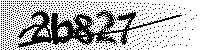
\includegraphics[width=0.25\textwidth]{./images/MA.png}};
\node (c) at (6.0,2.4) {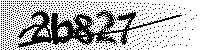
\includegraphics[width=0.25\textwidth]{./images/PE.png}};
\node at (-1.05, 3.2) {(Noisy Arc)};
\node at (1.9, 3.2) {(Modular Arithmetic)};
\node at (6.0, 3.2) {(Pixel Expansion)};
\end{tikzpicture}
\end{center}
In the case of Pixel Expansion implementation, the secret image ‘I’ is encoded as a binary string, where 0 represents a white pixel and 1 represents a black pixel. Each pixel from the secret image (Message to be encrypted) is sub-divided into more than one pixel i.e. each single pixel from the secret image is greater than one. Every single pixel in the secret image is encrypted using random selection of the possible permutation for all the sub pixel combinations.


\begin{center}
\putfigure{1.0\textwidth}{./images/vc-shares.png}
\textbf{Visual Encoding}
\end{center}

Modular Arithmetic method uses a grayscale image as input and converts it to black-and-white, essentially reducing the information contained within the image from 256 shades of gray to 2: black and white, a binary image. This is sometimes known as image thresholding, although thresholding may produce images with more than 2 levels of gray. It is a form or segmentation, whereby an image is divided into constituent objects.



\end{posterbox}

\begin{posterbox}[column=1, below=auto ]{4. Observation}

At first we use a deep learning based captcha solver to observe the detection rate of classic captchas. For this a classic CNN, namely LeNet-5 is applied.

% 
\hspace{0.1cm}

The training set contains 100,000 captchas and the testing set contains 10,000 captchas generated
by traditional captcha generation method.

%
\hspace{0.1cm}

When applying the deep learning-based breaking method to the above captchas, the success
rate is 95\%, which indicates that the traditional captchas are easily to be broke by deep learning-based
breaking method.





\end{posterbox}

\begin{posterbox}[column=2,]{5. Results}
The relevance of this proposed method is that the recognition rate is reduced significantly which makes the deep learning techniques hard to crack the captcha and thereby preventing unauthorized access.

\putfigureLR{0.50\textwidth}{./images/PE_cm.png}{0.50\textwidth}{./images/MA_cm.png}

\putfigurecaptionLR{0.45\textwidth}
{Pixel Expansion}

{0.45\textwidth}{Modular Arithmetic}


he accuracy and precision of the VC implementation models and the traditional Noisy Arc model is as given below:


\begin{center}

\begin{tabular}{||c c c c||} 
 \hline
 Type & Accuracy & Precision &\\ [0.5ex] 
 \hline\hline
 Noisy Arc & 92.75 & 93.26 & \\ 
 \hline
 Threshold VC & 53.83 & 44.55 & \\
 \hline
 Proposed VC & 27.81 & 44.31 & \\
 \hline
\end{tabular}
\end{center}

\end{posterbox}

\begin{posterbox}[column=2,below=auto]{6. Conclusion}

The relevance of this proposed method is that the recognition rate is reduced significantly which makes the deep learning techniques hard to crack the captcha and thereby preventing unauthorized access.Prediction of captchas by using deep learning is difficult when the captchas are enhanced by using VC.
%
\hspace{0.1cm}

By combining the above  two implementation methods we can reduce the recognition rates further and can take the security to the next level. 


\end{posterbox}


\begin{posterbox}[column=2, below=auto]{7. References}
1. Mengyun Tang,Haichang Gao,Yang Zhang and Ping Wang,”Research on Deep Learning Techniques in Breaking Text-Based Captchas and Designing Image-Based Captcha”,{\itshape IEEE Transactions on Information Forensics and Security}, 2018  Volume: 13, Issue: 10 ,Journal Article.

%
\hspace{0.1cm}

2. Suliman A. Alsuhibany, Meznah Alquraishi, “Usability and Security of Arabic Text-based CAPTCHA Using Visual Cryptography”, {\itshape Computer Systems Science \& Engineering, 2022}, DOI:10.32604/csse.2022.018929

%
\hspace{0.1cm}

3.Yan, X.; Liu, X.; Yang, C.N. An enhanced threshold visual secret sharing based on random grids. {\itshape Real-Time Image Process.} 2018, 14, 61–73

\end{posterbox}

\end{poster}
\end{document}
